\documentclass[11pt,a4paper]{article}

\usepackage[utf8]{inputenc}
\usepackage[T1]{fontenc}
\usepackage[spanish]{babel}

\usepackage{tgpagella}
\usepackage{geometry}
\usepackage{booktabs}
\usepackage{xcolor}
\usepackage{graphicx}
\usepackage{titlesec}
\usepackage{fancyhdr}
\usepackage[parfill]{parskip}
\usepackage[expansion=false]{microtype}
\usepackage{hyperref}
\usepackage{setspace}
\usepackage{needspace}
\usepackage{etoolbox}
\usepackage{ragged2e}

\widowpenalty=10000
\clubpenalty=10000
\displaywidowpenalty=10000

\hyphenpenalty=8000
\exhyphenpenalty=8000

\geometry{top=3.0cm,bottom=3.0cm,left=3.5cm,right=3.5cm}

\setlength{\parskip}{0.65em}
\setlength{\parindent}{0em}

\definecolor{azulai}{RGB}{30,80,140}
\definecolor{doradoai}{RGB}{140,90,0}
\definecolor{grisai}{RGB}{70,70,70}

\AtBeginDocument{\justifying}

\titleformat{\section}
{\Large\bfseries\color{azulai}\justifying}
{}
{0em}
{}
[{\color{azulai}\titlerule[0.5pt]}]

\titlespacing*{\section}
{0pt}{1.3em}{0.5em}

\titleformat{\subsection}
{\large\bfseries\color{doradoai}\justifying}
{}
{0em}
{}

\titlespacing*{\subsection}
{0pt}{1.0em}{0.35em}

\titleformat{\subsubsection}
{\normalsize\bfseries\color{grisai}\justifying}
{}
{0em}
{}

\titlespacing*{\subsubsection}
{0pt}{0.8em}{0.25em}

\preto\section{\Needspace{8\baselineskip}}
\preto\subsection{\Needspace{6\baselineskip}}
\preto\subsubsection{\Needspace{4\baselineskip}}

\pagestyle{fancy}
\fancyhf{}

\rhead{\textcolor{grisai}{\small dsf — Arquitectura Interna}}
\lhead{\textcolor{grisai}{\small Mercurio · Venus · Marte}}
\cfoot{\textcolor{grisai}{\small\thepage}}

\renewcommand{\headrulewidth}{0.3pt}

\hypersetup{
colorlinks=true,
linkcolor=azulai,
urlcolor=azulai
}

\setstretch{1.32}

\tolerance=1500
\emergencystretch=4em

\begin{document}

% ── Portada ──────────────────────────────────────────────────────────────────

\begin{titlepage}
  \centering

  \vspace*{2cm}

  {\Huge\bfseries\color{azulai} Mercurio · Venus · Marte}\\[0.6cm]

  {\large\color{grisai} Arquitectura Interna}\\[0.4cm]

  {\small\itshape\color{grisai}
  Procesamiento, vínculo y acción en el funcionamiento cotidiano
  }\\[2.2cm]

  {\huge\color{doradoai} dsf}\\[1.6cm]

  {\Large 16/08/1587 \quad 15:52}\\[0.35cm]

  {\Large fdas}\\[0.35cm]

  {\normalsize
  Lat: 14.5352° \quad
  Lon: 33.4504° \quad
  UTC+02:10
  }\\[0.35cm]

  {\normalsize
  Ascendente: Capricornio 15°44'
  \quad
  MC: Libra 25°06'
  }\\[2.2cm]

  \renewcommand{\arraystretch}{1.35}

  \begin{tabular}{ll}
    \textbf{Mercurio:} & Virgo — Casa 8 10°33' \\
    \textbf{Venus:}    & Cáncer — Casa 7 22°01' \\
    \textbf{Marte:}    & Escorpio — Casa 10 1°15' \\
  \end{tabular}

  \vfill

  {\small\color{grisai}
  Generado el 20/05/2026
  }

\end{titlepage}

\justifying

\tableofcontents

\clearpage

% ── Datos de referencia ───────────────────────────────────────────────────────
\section{Datos de referencia}

\begin{center}
\renewcommand{\arraystretch}{1.25}
\begin{tabular}{llll}
  \toprule
  \textbf{Planeta} & \textbf{Signo} & \textbf{Casa} & \textbf{Posición} \\
  \midrule
  Mercurio  & Virgo  & 8  & 10°33' \\
  Venus    & Cáncer & 7 & 22°01' \\
  Marte    & Escorpio & 10 & 1°15' \\
  Ascendente          & Capricornio           & ---                    & 15°44' \\
  Medio Cielo         & Libra            & ---                    & 25°06' \\
  \bottomrule
\end{tabular}
\end{center}
\justifying

\vspace{0.5cm}

\textbf{Aspectos entre planetas personales:}

\vspace{0.3cm}\textit{No hay aspectos entre los planetas personales en los orbes definidos.}

\justifying

\vspace{0.7cm}

\begin{center}
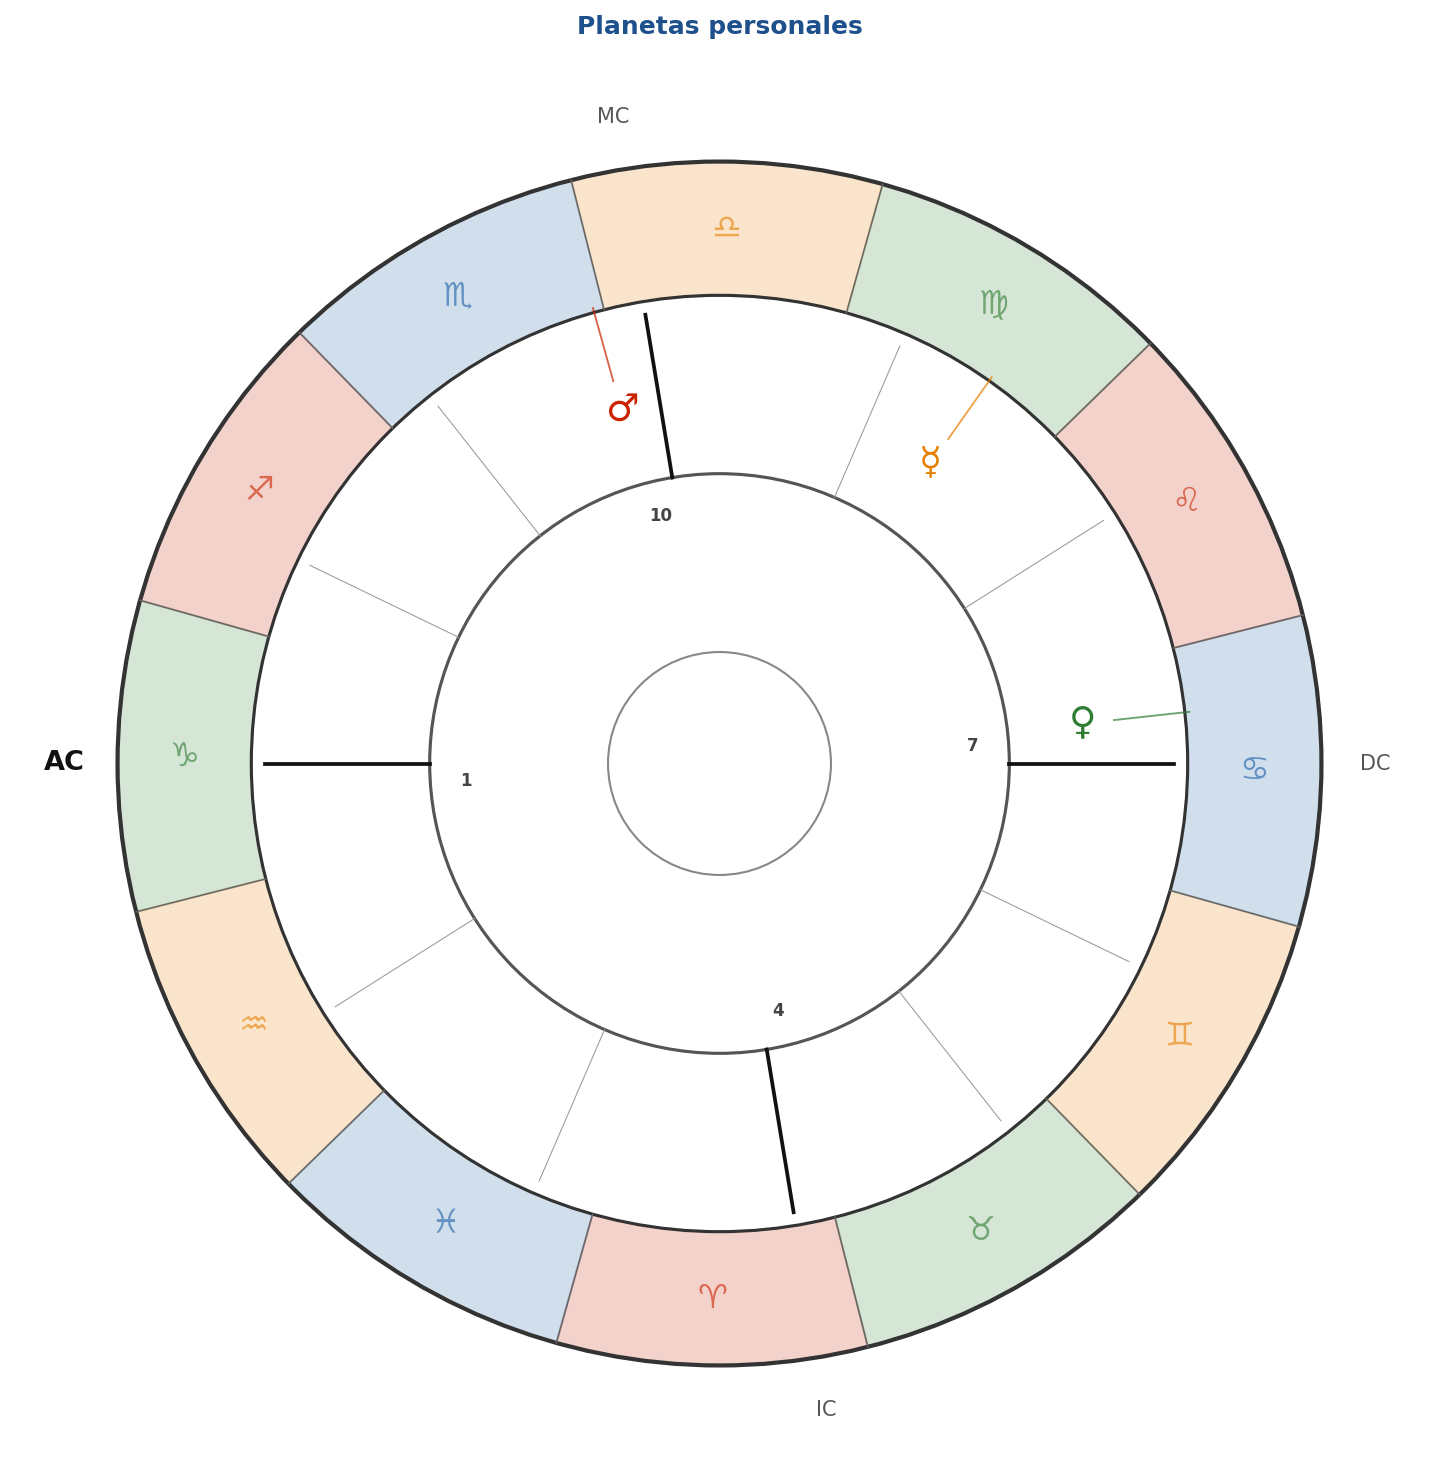
\includegraphics[width=0.72\textwidth]{dsf_Planetas_Personales_rueda.png}
\end{center}

\vspace{0.3cm}
\Needspace{5\baselineskip}

% ── Interpretación ────────────────────────────────────────────────────────────
\section{Interpretación — Arquitectura Interna}

\begin{center}
{\small\itshape\color{grisai}
No se trata de describir la personalidad.\\
Se trata de observar cómo procesas, cómo te vinculas\\
y cómo se mueve tu energía en la vida cotidiana.
}
\end{center}

\justifying

\vspace{0.8cm}

% ── 1. Funcionamiento general ─────────────────────────────────────────────────
\subsection{1. Funcionamiento general}

\justifying
Mercurio está en Virgo, Casa 8: muestra cómo piensas, cómo ordenas lo que percibes y cómo traduces lo que ocurre en palabras o ideas.
Venus está en Cáncer, Casa 7: muestra cómo te vinculas, qué necesitas para sentir conexión y cómo buscas equilibrio afectivo.
Marte está en Escorpio, Casa 10: muestra cómo se activa tu acción, cómo descargas energía y cómo respondes ante el impulso.

Hay coherencia elemental entre: tu forma de pensar (Mercurio) y tu forma de vincularte (Venus) se apoyan por elementos compatibles: Tierra/Agua; tu forma de pensar (Mercurio) y tu forma de actuar (Marte) se apoyan por elementos compatibles: Tierra/Agua; tu forma de vincularte (Venus) y tu forma de actuar (Marte) comparten elemento: Agua. Esto facilita que esas áreas colaboren entre sí. Aun así, lo que fluye con facilidad también puede volverse automático si no lo observas con consciencia.

No aparecen aspectos clásicos entre los planetas personales dentro de los orbes definidos. Aun así, puede existir una concentración funcional si los planetas están próximos por signo, por casa o por continuidad de experiencia.

\vspace{0.8cm}

% ── 2. Mercurio ───────────────────────────────────────────────────────────────
\subsection{2. Mercurio — Pensamiento y procesamiento}

\subsubsection*{Mercurio en Virgo — Casa 8}

\justifying
Tu mente funciona de forma analítica y orientada al detalle. Observas diferencias, detectas errores y tiendes a buscar cómo mejorar las cosas. Esto aporta precisión, capacidad de organización y atención a lo concreto.

La saturación aparece cuando el análisis nunca encuentra un punto de cierre. Siempre queda algo más por revisar, corregir o evaluar. Entonces aparece tensión mental de fondo y sensación de que nada termina de estar suficientemente acabado. El bloqueo típico es la parálisis por análisis: te cuesta actuar porque sientes que todavía faltan datos.

Sueles pensar mejor cuando existen estructuras simples, pasos claros y límites concretos para detener el análisis.

Tu mente tiende a profundizar y rara vez se conforma con explicaciones superficiales. Necesitas entender qué hay detrás: motivaciones, patrones, contradicciones o dinámicas ocultas. La comprensión suele requerir intensidad y profundidad para sentirse completa.

La saturación aparece cuando algo parece ambiguo o incoherente y no consigues comprenderlo del todo. Entonces puedes quedarte investigando internamente durante mucho tiempo. Sueles pensar mejor cuando tienes intimidad, silencio y conversaciones honestas donde puedas profundizar sin prisa.

\vspace{0.8cm}

% ── 3. Venus ──────────────────────────────────────────────────────────────────
\subsection{3. Venus — Vínculo y regulación relacional}

\subsubsection*{Venus en Cáncer — Casa 7}

\justifying
Necesitas cuidado mutuo, protección emocional y sensación de hogar compartido para sentirte en relación. La conexión suele fortalecerse cuando puedes mostrar vulnerabilidad sin miedo a perder el vínculo.

La saturación aparece cuando el cuidado deja de ser recíproco y empiezas a sostener emocionalmente más de lo que recibes. Entonces aparece agotamiento silencioso y cierre progresivo. Cuando el vínculo deja de sostenerse, no siempre te vas inmediatamente: a veces sigues presente mientras la apertura emocional real se va retirando.

Sueles regularte mejor en relaciones donde existe sensibilidad mutua, cuidado estable y seguridad emocional.

Las relaciones ocupan un lugar central en tu regulación afectiva. Necesitas reciprocidad clara, intercambio equilibrado y sensación de compromiso mutuo para sentir estabilidad.

La saturación aparece cuando existen relaciones ambiguas, desequilibrios prolongados o dificultad para definir el lugar de cada persona dentro del vínculo. Entonces puedes empezar a compensar demasiado al otro o perder estabilidad emocional. Sueles regularte mejor mediante acuerdos claros, diálogo y relaciones donde ambas partes sostienen conscientemente el vínculo.

\vspace{0.8cm}

% ── 4. Marte ──────────────────────────────────────────────────────────────────
\subsection{4. Marte — Acción y descarga}

\subsubsection*{Marte en Escorpio — Casa 10}

\justifying
Tu energía se activa con intensidad y concentración. Respondes con mucha fuerza cuando percibes amenaza, desafío o necesidad de transformación profunda. La acción descarga mediante enfoque, confrontación o procesos de cambio radical.

La saturación aparece cuando la energía queda acumulada sin salida clara. Entonces puedes entrar en estados de control excesivo, obsesión o activación interna permanente. La tensión retenida durante mucho tiempo puede descargarse de forma muy intensa cuando finalmente encuentra salida.

Sueles regularte mejor mediante actividad intensa, profundidad emocional y espacios donde puedas actuar con honestidad y enfoque.

Tu energía descarga mediante objetivos, ambición y construcción visible. Sueles activarte con fuerza cuando existe una dirección profesional, un reto concreto o algo que construir a largo plazo.

La saturación aparece cuando toda tu energía queda atrapada en exigencia, rendimiento o necesidad constante de sostener responsabilidad. Entonces puede aparecer dureza interna, dificultad para parar o sensación de vivir permanentemente en modo esfuerzo. Sueles regularte mejor mediante metas claras, estructura y tiempos reales de descanso.

\vspace{0.8cm}

% ── 5. Integración ────────────────────────────────────────────────────────────
\subsection{5. Integración — Coherencias, fricciones y bucles}

\justifying
Venus y Marte comparten elemento en Agua. Tu forma de vincularte y tu forma de actuar pueden colaborar con relativa facilidad. La energía disponible puede alimentar la relación, y el vínculo puede sostener el movimiento.

Cuando hay demasiada presión, puede aparecer una cadena reconocible: Mercurio en Virgo se fija en una posición y le cuesta actualizarla. Desde ahí, Venus en Cáncer absorbe el estado del entorno y pierde la referencia de lo que necesita. Y Marte en Escorpio se disipa o actúa en dirección del entorno antes que desde el propio impulso. El ciclo se cierra cuando la energía acumulada vuelve a saturar el punto inicial.

\vspace{0.8cm}

% ── 6. Orientación práctica ───────────────────────────────────────────────────
\subsection{6. Orientación práctica}

\subsubsection*{Desde dónde empezar}

\justifying
Desde tu forma de pensar (Mercurio) en Virgo, Casa 8. De las tres áreas, esta suele requerir menos energía para activarse. La entrada es llevarlo a una acción concreta, pequeña y verificable. Empezar por aquí puede abrir movimiento en el resto.

\subsubsection*{Qué sostener}

\justifying
Conviene sostener especialmente tu forma de vincularte (Venus) en Cáncer: tiempo de integración, silencio emocional y límites sensibles. Bajo presión, esta área puede desorganizarse antes que las demás. Cuando se estabiliza, el resto de tu funcionamiento tiene más capacidad para reorganizarse.

\subsubsection*{Qué evitar}

\justifying
Evitar asumir que la ausencia de fricción visible significa que todo está bien. A veces los bucles no hacen ruido porque te has acostumbrado a funcionar así.

\vspace{0.6cm}

\justifying
Si no se sostiene: pensamiento, vínculo y acción empiezan a funcionar por separado. Lo que piensas no alimenta la acción, la acción no informa al vínculo y el vínculo no regula la energía disponible. El esfuerzo aumenta, la claridad disminuye y la saturación llega antes.

\vspace{1.2cm}

\begin{center}
{\small\itshape\color{grisai}
La astrología se utiliza aquí como lenguaje simbólico de observación,\\
no como una definición cerrada de quién eres.\\[0.2cm]
Este documento propone una lectura funcional y orientativa, no un diagnóstico.
}
\end{center}

\end{document}
